\chapter{Metodología}
\label{chap:metodologia}

En este capítulo se describen las bases teóricas y técnicas del modelo de distribución de la luz en la atmósfera \textit{SkyGlow} desarrollado por \cite{Kocifaj2007}, además del software \textit{Radiance Light Trends} desarrollado por \cite{RLT2019} que permite analizar datos de radiancia medidos por el sensor \textit{Visible Infrared Imaging Radiometer Suite} (VIIRS) a bordo del satélite \textit{Suomi National Polar-orbiting Partnership}.\\

Advertencia: la distribución de radiancia teórica generada por el modelo \textit{SkyGlow} se construye considerando un observador en superficie por lo que, al comparar los valores de radiancia teóricos del modelo con los generados por el VIIRS, no se pretende validar el modelo, sino estimar la tendencia de los valores de radiancia para el área de interés.\\

En el \textbf{\autoref{chap:recomendaciones}} se presentan propuestas para validar el modelo \textit{SkyGlow} para la Ciudad de México.\\ 

\section{El modelo \textit{SkyGlow}}


\textit{SkyGlow} es un modelo teórico escalable que permite simular el comportamiento angular de la radiancia en el cielo durante la noche en una región específica o integrada del EE. No considera restricciones en el número de fuentes de luz ni en la distribución espacial de las mismas en la vecindad del punto de medición, por lo que la distancia y el ángulo acimutal de las fuentes de luz son configurables. El modelo es aplicable para fuentes de luz con dimensiones finitas reales con propiedades radiativas espectrales y angulares definidas \citep{Kocifaj2007}.\\ 

La influencia de la atmósfera en la modulación de la radiación es formulada en términos de propiedades ópticas de las moléculas de aire y aerosol atmosférico. La reflectancia espectral y la altitud de las capas de nubes son los principales factores tomados en cuenta para la modelación de condiciones de nubosidad \citep{Kocifaj2007}, \citep{Solano2014}.\\ 

Las ecuaciones derivadas son traducidas en código numéricamente rápido, lo que es deseable para la realización de experimentos numéricos que incluyen una malla con gran número de puntos (dominio geográfico grande con alta resolución espacial) \citep{Kocifaj2007}, \citep{Linares2018}.\\

\subsection{Datos de entrada}

\textbf{Definición del dominio}

El área de la superficie de estudio (forma y tamaño) es definida a través de vértices coordenados (latitud y longitud). \textit{Para este estudio}: polígonos de cada una de las 16 alcaldías de la Ciudad de México y de la REPSA (Figura~\ref{ciudaddemexicomodelo}).

\newpage

\begin{figure}
  \centering
    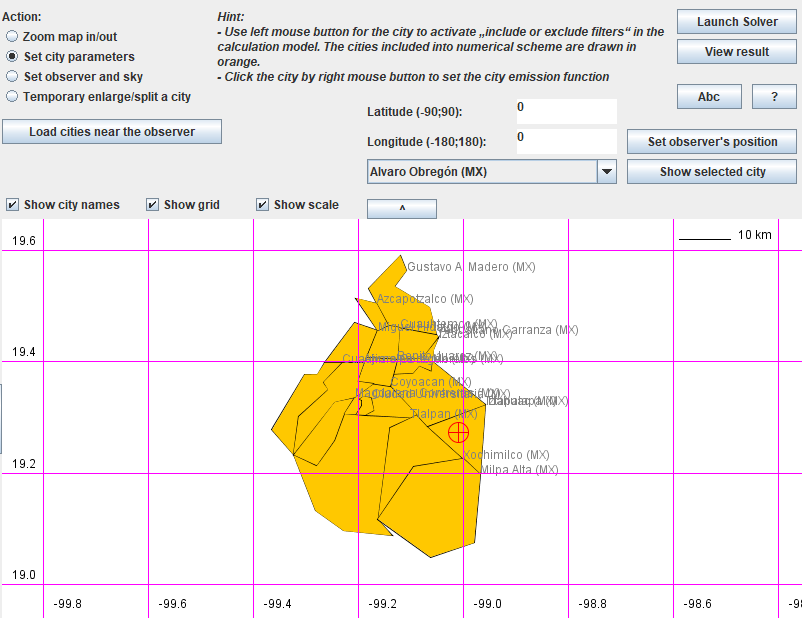
\includegraphics[width=0.6\textwidth]{ciudaddemexicomodelo}
  \caption{Intefaz gráfica del modelo \textit{SkyGlow}}
  \label{ciudaddemexicomodelo}
\end{figure}

\textbf{Inventario de fuentes de luz}

El modelo calcula la emisión total de las fuentes de luz con base en la población (típicamente 750 lm por habitante) y su dependencia espectral \textit{Para este estudio}: datos del \textbf{Inventario de Alumbrado Público de la Ciudad de México} (Tabla \ref{tab:inventariocdmx}).\\

\textbf{Variables del caso de estudio}

Una vez que el escenario está definido, el modelo requiere de parámetros específicos del experimento numérico que se desarrollará:

\begin{itemize}

    \item Rango de longitud de onda: la máxima y mínima longitud de onda a estudiar. \textit{Para este estudio}: rango visible del EE dividido en 40 ventanas de 10 nm, con el fin  de estimar el efecto de la dependencia espectral de las fuentes de luz reportadas en el \textbf{Inventario de Alumbrado Público de la Ciudad de México}.
    
    \item Aerosol atmosférico: véase la \textbf{\autoref{subsubsec:propiedadesopticasaerosol}}. \textit{Para este estudio}: los experimentos numéricos se realizaron considerando la climatología descrita en la \textbf{\autoref{subsec:climatologia}}. Para condiciones de fondo promedio (FP) se considera el Espesor Óptico de Aerosol AOD = 0.1, Parámetro de Angstrom $\alpha$ = 1.3, Parámetro de Asimetría ASY = 0.6 y Albedo de Dispersión Simple SSA = 0.85; Para especies carbonosas (EC, carbón elemental producto de la combustión incompleta de combustibles fósiles y carbón orgánico) AOD = 0.1, $\alpha$ = 1.3, ASY = 0.3, SSA = 0.3. (Todos los parámetros constantes a lo largo del espectro estudiado) \citep{Penner1998}, \citep{Schmidt2010}.
    
    \item Nubosidad: altura y albedo espectral de la capa de nube. \textit{Para este estudio}: véase la \textbf{\autoref{subsec:climatologia}}
    
    \item Posición del observador: en coordenadas (latitud y longitud) 
    
\end{itemize}

\subsection{Bases teóricas del modelo}

La intensidad de la luz que crea el patrón del brillo del cielo en un volumen atmosférico elemental es la suma de todas las intensidades de todos los rayos emitidos de diferentes áreas en diferentes ángulos cenitales. \cite{Kocifaj2007} expresa la radiancia espectral (W sr$^{-1}$  m$^{-2}$ nm$^{-1}$) del cielo despejado como:

\begin{equation}\label{eq:2.1}
I_{\lambda}(z, \phi) = \frac{A_{0}\, S_{\lambda}}{cos\,z} \int_{h=0}^{h} B_{\lambda}(Q, q, z') \: \Gamma_{\lambda} \:(h, z, \phi, z', \phi') \: T_{\lambda}(h, z, \phi) \: \frac{cos^{2}z'}{h^{2}} dh
\end{equation}

Donde $\lambda$ es la longitud de onda a la que se emite la luz, $z'$ y $\phi'$ son el ángulo cenital y acimutal de la luz emitida respectivamente, mientras que $z$ y $\phi$ caracterizan la posición del elemento de cielo observado y h es su altura con respecto al observador P (Figura~\ref{geometriamodelo}).\\

El primer término de la izquierda de la ecuación captura la emisión de las fuentes de luz (no dependen del observador) donde $A_{0}$ es un elemento de superficie de una fuente de luz que radia en todas direcciones y $S_{\lambda}$ es la potencia emitida por elemento de superficie $A_{0}$ de la fuente radiante (W m$^{-2}$ nm$^{-1}$).\\


\begin{figure}[htb]
  \centering
    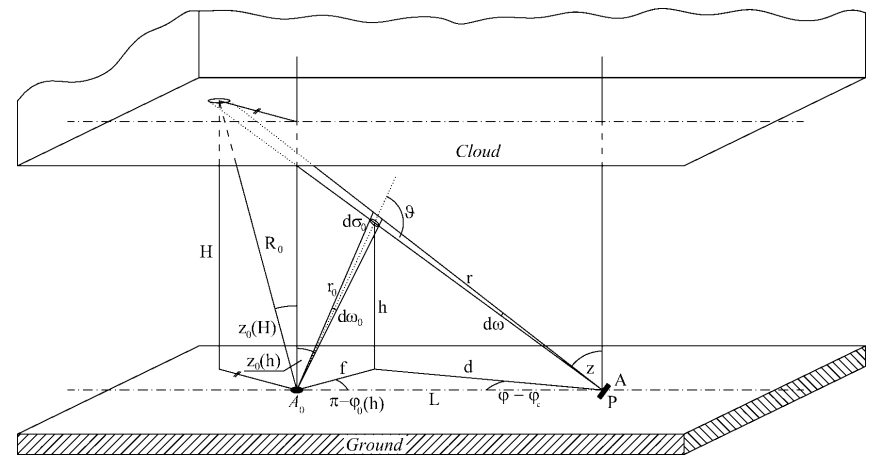
\includegraphics[width=1\textwidth]{geometriamodelo}
  \caption{Geometría del modelo \citep{Kocifaj2007}}
  \label{geometriamodelo}
\end{figure}


Los procesos capturados por los términos dentro de la integral se desarrollan en la atmósfera (por ello están integrados desde la superficie hasta la altura h). $B$ es la Función de Emisión Urbana (CEF) abordada en la \textbf{\autoref{subsec:climatologia}}, esta función determina el comportamiento angular de la radiación emitida por las fuentes de luz; la aproximación semi-empírica a la CEF que \cite{Garstang1986} (Garstang Emission Function, GEF) desarrolló es:

\begin{equation}
B(Q, q, z') = 2Q(1-q) cos \, z' + 0.554q \,z'^{4}
\end{equation}

Donde $Q$ es la fracción de la luz que es reflejada isotrópicamente desde la superficie y $q$ es la fracción radiada directamente hacia arriba, con respecto al ángulo cenital $z'$. La \textbf{Tabla \ref{tab:valoresdeq}} muestra los valores de q utilizados para este estudio.


\begin{table}[htb]
\centering
\caption{Fracción $q$ radiada directamente hacia arriba en el ángulo cenital $z'$ \citep{Kocifaj2007}}
\label{tab:valoresdeq}
\resizebox{0.5\textwidth}{!}{%
\begin{tabular}{|c|c|c|c|c|c|c|c|c|c|c|}
\hline
\textbf{z'} & 0 & 10 & 20 & 30 & 40 & 50 & 60 & 70 & 80 & 90 \\ \hline
\textbf{q} & 1 & 0.95 & 0.8 & 0.7 & 0.6 & 0.5 & 0.4 & 0.3 & 0.15 & 0 \\ \hline
\end{tabular}%
}
\end{table}

Resulta importante mencionar que \cite{Kocifaj2016} señalan la falta de validez de la GEF en algunos casos. La GEF sobrestima las emisiones en ángulos cenitales bajos debido a que estas son fácilmente suprimidas por obstáculos.\\

 Sin embargo, ya que el modelo \textit{SkyGlow} está basado en el Método de Órdenes de Dispersión Sucesivos (MODS)\footnote{El MODS modela la intensidad de una señal dispersada a través de una expansión en serie de varios órdenes sucesivos. \textit{SkyGlow} únicamente toma el primer orden de la serie (dispersión simple) \citep{USENERGY2017}} con fuentes de tamaño finito, las deficiencias de la GEF no resultan críticas \citep{USENERGY2017}.\\

Continuando con el análisis de la ecuación \ref{eq:2.1}, $\Gamma$ es una función que caracteriza la distribución angular de la luz dispersada de un volumen elemental de la atmósfera en una altura $h$. Se calcula como el producto del coeficiente de dispersión y la función de fase de dispersión (véase la \textbf{\autoref{subsubsec:propiedadesopticasaerosol}}). $\Gamma$ varía con el ángulo de dispersión $\vartheta$ en $h$, que a su vez depende de la dirección de observación, la dirección de los rayos emitidos y la distancia $L$ entre la fuente de luz y el observador:

\begin{equation}
cos \, \vartheta_{h} = \frac{1}{2} \left(\frac{L^{2}}{h^{2}} \: cos \, z \: cos \, z' - \frac{cos \, z'}{cos \, z}- \frac{cos \, z}{cos \, z'}\right)
\end{equation}


Por último, $T$ es una función que caracteriza la atenuación atmosférica en términos del AOD:

\begin{equation}
T_{\lambda}(h, z, \phi) = t_{\lambda}(h,z) \, t_{\lambda}(h, z')
\end{equation}

Si la radiancia espectral $I_{\lambda}(z, \phi)$ es conocida, entonces la irradiancia espectral difusa en una superficie horizontal $D_{\lambda}$ puede ser calculada \citep{Kocifaj2014} como: 

\begin{equation} \label{eq:2.5}
D_{\lambda} = \int_{z = 0}^{z =\pi/2} \int_{\phi = 0}^{\phi = 2\pi} I_{\lambda} (z, \phi) \: sen \,z \: dz \: d\phi
\end{equation}

Para el caso en que se considera cielo nublado, se suma a la ecuación \ref{eq:2.1} el término de la interacción del flujo de luz con una capa nubosa a una altura $H$:

\begin{equation} \label{eq:2.6}
I_{\lambda, Nube}(z, \phi) = S_{\lambda} \: \frac{A_{0} \, \rho_{\lambda}(z'_{H}, z, \vartheta_{H})}{\pi H^{2}} \: B_{\lambda}(Q, q, z'_{H}) \: T_{\lambda}(H, z, \phi) \: cos^{4} \, z'_{H}
\end{equation}

Donde $\rho$ es la reflectancia espectral de la nube, $z'_{H}$ es el ángulo cenital de la luz emitida con respecto al elemento de área radiante de la nube y $\vartheta_{H}$ es el ángulo de dispersión en $H$. Sumando la ecuación \ref{eq:2.1} y \ref{eq:2.6} se obtiene la expresión para la radiancia espectral total con cielo nublado $I_{\lambda, Total}(z, \phi)$.

\newpage

Considerando que el punto del observador está rodeado de $N$ fuentes de luz, donde la características radiativas de la $i$ésima fuente son $S_{i}$, $Q_{i}$, $q_{i}$ y la distancia y el ángulo acimutal de la $i$ésima fuente son $L_{i}$ y $\phi_{i}$ respectivamente. La cantidad total de la intensidad de la luz dispersada es calculada como la suma de todas las fuentes: 

\begin{equation}
J(z, \phi) = \sum_{i=1}^{N} \int_{\lambda_{1}}^{\lambda_{2}} I_{\lambda, i}(z, \phi)  \: d\lambda
\end{equation}

\subsection{Visualización de datos de salida}

Las salidas del modelo son:

\begin{itemize}


	\item irradiancia espectral (W m$^{-2}$) difusa en una superficie horizontal

	\item radiancia (W m$^{-2}$ sr $^{-1}$) en $z$ ($0\grad - 85\grad$), $\;$  $\phi$ ($0\grad - 360\grad$)

    
\end{itemize}



\textbf{Gráficas tipo \textit{all-sky}}\\

La distribución de la radiancia integral en el cielo se visualiza con gráficas polares del logaritmo de las salidas de radiancia del modelo (Figura~\ref{graficapolar}). Estas gráficas se interpretan como la radiancia que llega a un observador desde todas las partes del cielo (180\grad), por lo que son denominadas gráficas tipo \textit{all-sky}. El ángulo a lo largo del círculo representa el ángulo acimutal $\phi$ mientras que el ángulo cenital $z$ es medido desde el centro hasta el margen de la gráfica.\\

El código fue desarrollado por el Dr. Miroslav Kocifaj de la Academia Eslovaca de Ciencias en gnuplot y está integrado en el modelo \textit{SkyGlow}.\\


\begin{figure}[htb]
  \centering
    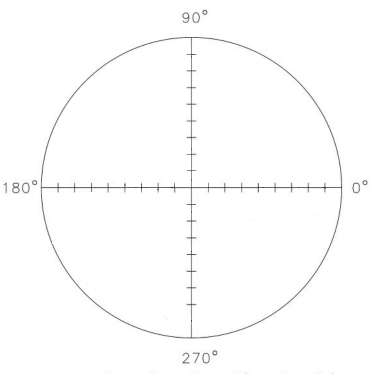
\includegraphics[width=0.3\textwidth]{graficapolar}
  \caption{Gráfica polar}
  \label{graficapolar}
\end{figure}\\


\textbf{Mapa coroplético}}\\

El \textbf{Mapa Teórico de Contaminación Lumínica de la Ciudad de México} (Mapa CL-CDMX) es un mapa coroplético de irradiancia espectral difusa en una superficie horizontal calculada con \textit{SkyGlow} con condiciones de FP. El código desarrollado en Julia se presenta en el \textbf{\autoref{chap:anexos}}. Los polígonos de sectores de la Ciudad de México se obtuvieron de la página de Datos Abiertos Ciudad de México (\url{datos.cdmx.gob.mx}}) y se tradujeron al formato TopoJSON con la biblioteca de software GDAL.

\newpage

\section{El software \textit{Radiance Light Trends}}

\textit{Radiance Light Trends} es una aplicación web (\url{lighttrends.lightpollutionmap.info}}) que permite analizar tendencias mundiales de radiancia promedio desde 2013 hasta la fecha con datos satelitales nocturnos de la banda Día/Noche (DNB) del VIIRS, disponibles en la página \textit{National Centers for Environmental Information} (\url{https://ngdc.noaa.gov/}}) de la \textit{National Oceanic and Atmospheric Administration} (NOAA).\\

\subsection{Especificaciones}

La banda DNB de la VIIRS está especialmente diseñada para observar la luz artificial a escala mundial. Escanea una región alrededor de la 1:30 am en un rango espectral de 500-900 nm con una resolución espacial de 0.5 km$^2$ \citep{Elvidge2017}.\\

\subsection{Consideraciones}

Las imágenes producidas por DNB son filtradas para reducir ruido de fondo, contaminación de radiancia debida a la luz solar y lunar y cobertura nubosa. Sin embargo, pueden observarse variaciones en corto plazo (meses) debido al ángulo de las imágenes con que se hacen las composiciones mensuales, incendios, fuegos artificiales y bengalas. Debido a esto, resulta recomendable analizar los datos de DNB en tendencias a largo plazo (anuales) para centrarse en las variables de interés: la variación de la radiancia debido al cambio de los sistemas de iluminación (número, fuente y distribución espacial) \citep{Coesfeld2018}, \citep{Elvidge2017}.\\

\subsection{Productos}

La aplicación calcula para cada polígono de cada alcaldía de la Ciudad de México la radiancia promedio anual y le ajusta una línea de tendencia exponencial y una máscara cuando la región es mayor a 100 km$^2$. Además, la interfaz gráfica de la aplicación permite visualizar una composición de imágenes de DNB de radiancia promedio para el 2016 (Figura~\ref{radiancetrends}) en la que, cualitativamente, las regiones más claras indican valores más altos de radiancia.

\begin{figure}[htb]
  \centering
    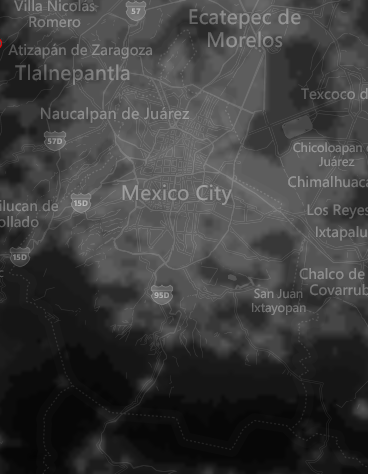
\includegraphics[width=0.3\textwidth]{RadianceTrends}
  \caption{Composición de imágenes satelitales de radiancia en la Ciudad de México (imagen y datos procesados por la NOAA, bajo los términos de uso de Microsoft\textregistered \: Bing\textsuperscript{TM} \: Maps Platform)}
  \label{radiancetrends}
\end{figure}